\documentclass[11pt,sigconf]{acmart}

\usepackage{booktabs} % For formal tables

\graphicspath{{figure/}{figures/}}

% Copyright
%\setcopyright{none}
%\setcopyright{acmcopyright}
%\setcopyright{acmlicensed}
\setcopyright{rightsretained}
%\setcopyright{usgov}
%\setcopyright{usgovmixed}
%\setcopyright{cagov}
%\setcopyright{cagovmixed}


% DOI
\acmDOI{10.475/123_4}

% ISBN
\acmISBN{123-4567-24-567/08/06}

%Conference
\acmConference[CSCI-5502 '21]{CSCI-5502 Data Mining Summer 2021}{July 2021}{Boulder, CO, USA} 
\acmYear{2021}
\copyrightyear{2021}

\acmPrice{15.00}


\begin{document}
\title{CSCI 5502 Project Proposal}
\titlenote{This proposal is Part 2 of the CSCI-5502 Data Mining Project}
\subtitle{The Pandemic within COVID-19: Assessing Misinformation Susceptibility}

\author{Son Pham}
\orcid{1234-5678-9012}
\affiliation{%
  \institution{CU Boulder}
  \streetaddress{Address}
  \city{Boulder} 
  \state{Colorado} 
  \postcode{80309}
}
\email{son.pham-2@colorado.edu}

\author{Kyle Rogers}
\orcid{1234-5678-9012}
\affiliation{%
  \institution{CU Boulder}
  \streetaddress{Address}
  \city{Boulder} 
  \state{Colorado} 
  \postcode{80309}
}
\email{kyro3301@colorado.edu}

\author{Reiko Matsuda-Dunn}
\orcid{1234-5678-9012}
\affiliation{%
  \institution{CU Boulder}
  \streetaddress{Address}
  \city{Boulder} 
  \state{Colorado} 
  \postcode{80309}
}
\email{rema8973@colorado.edu}

\author{Ryan Karasopoulos}
\orcid{1234-5678-9012}
\affiliation{%
  \institution{CU Boulder}
  \streetaddress{Address}
  \city{Boulder} 
  \state{Colorado} 
  \postcode{80309}
}
\email{ryka6853@colorado.edu}


% The default list of authors is too long for headers}
\renewcommand{\shortauthors}{S. Pham, K. Rogers, R. Matsuda-Dunn, and R. Karasopoulos}


\begin{abstract}
This paper focuses on how COVID-19 information was communicated within and between different countries, reactions of governments to the pandemic, and attitudes and risk perceptions people had towards the virus. The major questions to answer are how digital communications influenced people’s interpretation of the news, what their responses were to the new laws and mandates, their beliefs and concerns regarding the pandemic versus other world issues, and the similarities and trends among the different countries.
\end{abstract}

%
% The code below should be generated by the tool at
% http://dl.acm.org/ccs.cfm
% Please copy and paste the code instead of the example below. 
%
\begin{CCSXML}
<ccs2012>
   <concept>
       <concept_id>10002951.10003317.10003359.10011699</concept_id>
       <concept_desc>Information systems~Presentation of retrieval results</concept_desc>
       <concept_significance>500</concept_significance>
       </concept>
   <concept>
       <concept_id>10002950.10003648</concept_id>
       <concept_desc>Mathematics of computing~Probability and statistics</concept_desc>
       <concept_significance>300</concept_significance>
       </concept>
   <concept>
       <concept_id>10002951.10002952</concept_id>
       <concept_desc>Information systems~Data management systems</concept_desc>
       <concept_significance>500</concept_significance>
       </concept>
   <concept>
       <concept_id>10002951.10002952.10003219</concept_id>
       <concept_desc>Information systems~Information integration</concept_desc>
       <concept_significance>500</concept_significance>
       </concept>
   <concept>
       <concept_id>10002951.10002952.10002953</concept_id>
       <concept_desc>Information systems~Database design and models</concept_desc>
       <concept_significance>500</concept_significance>
       </concept>
 </ccs2012>
\end{CCSXML}

\ccsdesc[500]{Information systems~Presentation of retrieval results}
\ccsdesc[300]{Mathematics of computing~Probability and statistics}
\ccsdesc[500]{Information systems~Data management systems}
\ccsdesc[500]{Information systems~Information integration}
\ccsdesc[500]{Information systems~Database design and models}

% We no longer use \terms command
%\terms{Theory}

\keywords{Data Mining, COVID-19, Risk Perception, Communication, Misinformation}


\maketitle


\section{Introduction}

The worldwide pandemic known as the corona virus disease 2019 (COVID-19) placed the world under lockdown and greatly changed the global perception of the veracity of trustworthy sources and how information is presented. Various influences ranging from social media and local news depictions of the virus to a lack of trust by individual and political actors have cultured an environment that facilitates the frequent spread of misinformation. In this study, we will examine survey data from 12 different countries across the globe conducted by Roozenbeek et. al. \cite{roozenbeek}. The responses to the provided questions are coupled to form predictions on the level of individual comprehension relating to COVID-19. Elements such as trust in various entities, questions pertaining to personal feelings of risk, and basic informal personal questions allowed for an assessment of collective misunderstanding across a diverse range of surveyed countries.

\subsection{Motivation}
%Go in detail about the problem statement and motivation.

The general spread of misinformation in modern society is an interesting and important topic. Acceptance of misinformation as truth can influence critical outcomes such as election results, public trust, and public health. This data set not only contains information that may help explain the mechanism behind the spread of misinformation regarding COVID-19, but the intersection of these fields.

%\begin{figure}[htbp]
% \centering
%  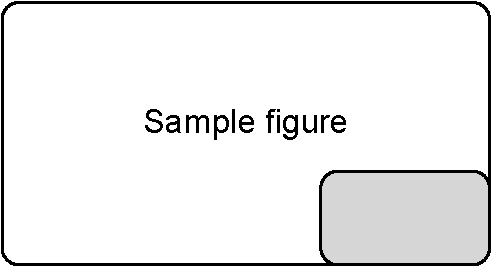
\includegraphics[scale=0.5]{figure1}
%  \caption{Sample figure}
%  \label{fig:sample}
%\end{figure}

%\subsubsection{Subsubsection if needed}



\section{Literature Survey}
%Describe and site all any literature found.

A vigorous literature survey was conducted to ensure the authors' analyses remain illustrating original and interesting results. This was broken down into two parts: studies outside of the data set that assessed mental health and collaboration amidst COVID-19, and studies done on parts of the data set.

%Original paper: https://royalsocietypublishing.org/doi/\newline10.1098/rsos.201199#d1e2648 %will need to add proper citation

\subsection{External studies}

Given the urgent and drastic nature of COVID-19, there are many publications and corresponding data sets available. This study wanted to focus on data outside of the more common death rate, positive test rate, and overall case rate data sets. As such, data regarding mental health and perceptions was a focus of this study. One article of interest involved collaboration analysis between countries as a result of COVID-19 \cite{roozenbeek}. A strengthened bilateral research relationship was evident between multiple countries, and the study identified the US, UK, and China as the largest contributors to COVID-19 research. Another article of interest observed psychological effects from COVID-19 in Spain \cite{rodriguezrey}. Survey data was collected during the initial stages of the pandemic and was given a rating on the Impact of Event scale, which assesses psychological distress caused by a traumatic life event.

\subsection{Studies based on this data set}

Prior work concluded that a belief in COVID misinformation was rare, however this type of misinformation is often perceived as highly reliable by a small but persistent  cohort. Higher trust in science and math abilities were associated with lower susceptibility to misinformation. Researchers used basic statistical methods such as ANOVAs and ordinary least squares (OLS) linear regression to evaluate survey results \cite{roozenbeek}. Significant differences were found in the perceived reliability of misinformation between countries. Linear regression found that predictors of susceptibility to misinformation included identifying as politically right-wing, self-identifying as a member of a minority group, and using social media as a source of information. Predictors of lower susceptibility to misinformation include trust in scientists and higher numeracy (math) scores.

Another publication for the data set focuses on risk perceptions of the surveyed individuals \cite{dryhurst}. This study involves 10 of the 12 countries from the original study. Based on van der Linden's (2015, 2017) risk perception model, the questions from the survey are grouped based on mental and emotional experiences, the social-cultural perception of risk, and relevant individual differences. This publication highlights some of the main factors contributing to risk perception, as well focus on the most apparent risk-prone countries involved in the study. 
%curious about self-identified minority groups: It's categorized as ethnic minority but the question is "Do you consider yourself to be part of a minority group within the country you are currently living in?" (unclear if participants saw that this was intended as an ethnic minority). Largest positive correlation is in Ireland, next largest is Mexico. 

\section{Proposed Work}
% What do you need to do for data collection, pre-processing (cleaning, integrating, transforming, etc.) processing for derived data, design, evaluation...
% Describe how it is different that what has been done previously from your literature survey (or if replicating).

One published paper for this data set reviews survey results from five different countries: The UK, Ireland, the United States, Mexico, and Spain. However, data on twelve different countries was collected, the seven additional countries being China, Sweden, Japan, Korea, Italy, Australia, and Germany. We will examine the complete data set as well as correlations of different survey results via clustering and other classification techniques (i.e. using the holdout method to determine classifiers).
%I think the hold out method is to verify created models, not to determine classifiers? --Reiko
While previous literature has provided correlations of the survey data, there is much room for additional study.

This study would also like to implement techniques similar to those used by Dryhurst et. al. to cluster the data presented and potentially identify a numeric metric for misinformation related to COVID-19 \cite{dryhurst}. This numerical value would be utilized in a similar nature to the ranking of individuals on the Impact of Event scale. This could allow relation of traumatic events and misinformation. %really not sure what i'm trying to say here

%Stretch goal: examine the relationship between the people who expressed reservations in getting the vaccine at the time of this study (surveyed April-May 2020) vs. percent currently vaccinated in the US (focus on US because the roll out here has been faster than Europe, though unsure about rate of roll out in Asia and Australia, which could possibly be better options/examined in addition).

\subsection{Data Cleaning and Pre-processing}

Given the data will be processed using Python, each data set will be imported from the available comma-separated values files (csv's) into Pandas DataFrames. String data and integers will be mostly used, with some attributes requiring float precision. Filtering of participants who did not accurately report their results (i.e. someone submitting all 7's or all 1's) will be accounted for as well. There will also be additional filtering of null values, which will be assessed as valid or invalid to the survey data.

\subsection{Data Integration}

The first steps of the data integration involve combining the different data sets into one complete set. This is accomplished more easily via consistent attribute naming, which is done in the data pre-processing phase. As some attributes are of the same name but different survey categories, a set method is to be used to differentiate these attributes. 

\subsection{Statistical Analysis and Decision Trees}

The first analysis will be to explore statistical information of the dataset. Although most of the attributes are either nominal or ordinal, statistical analysis may be useful for the available numerical attributes. Parameters such as mean, median, mode, range, and quantiles will help summarize the dataset where logical do to so.

Another data mining technique is to determine the similarities and dissimilarities between object groups relative to the attributes of the dataset. This process can be performed on any type of attribute and, for the dataset in focus, it may be possible to be performed on a mixed set of attributes. These techniques may be effective at showing how alike or unalike people surveyed in certain countries are in comparison to others. Measuring similarity and dissimilarity will lead to clustering technique which will be discussed in the next section.

A third method of analyzing the data will be to create a decision tree model that could predict categorical labels among the different attributes. Information gain selection will be performed to determine the best attributes to split on and help make the decision trees as effective as possible. This technique may help determine the potential attributes that may be behind scenarios such as the mechanisms that influence the spread of misinformation and the probabilities of one perception affecting another.

\subsection{Data Clustering and Presentation}

For the COVID-19 survey data analyzed we will be performing clustering on various sets of attributes. We will target differences in perceptions of COVID-19 risks by country, so residency will be an attribute that will be important to attempt to incorporate. Survey data such as education level and numeracy scores will be interesting attributes to cluster on. It will be important to first identify if there is a correlation between these attributes and select one or the other accordingly. Trust in scientists, journalists, and government responses will be other important attributes to include in the model. It is expected that many iterations of the clustering model will be performed, and not all attributes will lead to interesting results, so some may ultimately be omitted. 

Results will be visualized with histograms for each clustered category and scatter plots to map clusters. An interactive visualization using Plotly will be a potential stretch goal. Possibilities include a dashboard that incorporates maps to demonstrate trends across countries.

\section{Data Set}
%Make sure you have the data set!. Provude URL and details about the data set (similar to hw1, ch2, etc)

The dataset is available from https://osf.io/vhnk7/, which includes survey answers from ten thousand participants across eleven different countries. These survey questions include demographic data (seven attributes), 90 questions regarding perceptions of COVID-19 risks, preparedness, information sources, trust in society, political views, and four probability math questions. The final analysis results of the original researchers is also provided. This includes ordinal scores for several categories such as "Trust in government" or "Trust in journalists" summarized from survey results. 

The primary data (i.e., original survey answers) is available in fifteen separate csv files (separated by country). There are several different formats among these csv files, so some integration was required. After the initial integration, 12,820 objects were assembled in the data set.

\section{Evaluation Methods}

Evaluation methods will include a brief review of summary statistics, clustering, and visualization. The former will consist of a correlation analysis to compare individual categories in survey results. The original study relied on multiple linear regression and an ANOVA to produce results for five countries. While this project will examine all 12 countries surveyed, an important component of this process will be to avoid repeating this work, but it is expected that new results should support those of the original study. These correlation results will inform the selection of attributes used for clustering.

Clustering analysis will be performed to discover trends based on country, education level, and survey answers. This will likely provide the bulk of the project results. Clustering results could be evaluated by retaining a portion of the data set as a test set. Standard metrics such as accuracy, sensitivity, specificity, and precision can be used to quantify this evaluation.

Because we will also be looking into decision tree analysis, the two models can be compared and possibly merged.

An additional stretch goal is to analyze longitudinal results. A small (just under 6280 objects), longitudinal dataset is provided from the same source. This contains survey data collected two months after the first survey and could be used to supplement this work. Additionally, known population responses by country could be investigated. This would require finding a dataset from an additional source, and assuming that our samples are equally representative of the population as a whole. This final step could determine if misinformation susceptibility, as determined by our model, is a predictor of a measurable response such as vaccination rate.

\section{Tools}

As mentioned previously, Python will be the primary resource utilized by the team. This will involve the use of various IDE's across the team, as well as many libraries constructed for Python. These libraries include NumPy (for computations and array manipulation), Pandas (for data manipulation and DataFrame creation), Scikit-Learn (for clustering), Plotly (for plotting and visualization), and potential use of Tkinter (for user interface options). Git and GitHub are used in conjunction  for a version-controlled communal code repository, allowing team members to record and review respective version histories and commits. Additional tools include Overleaf for an online interface for group participation in report generation, and Google Documents/Sheets/Presentations for group interaction and further collaborative efforts.

\section{Milestones}

Each group member will be involved in completing parts of the study. A detailed milestone assessment has been developed to ensure proper communication and completion throughout the study. The dates laid out below are targeted completion dates.\\

\subsection{Week of June 21st - Project Part 1: Project Proposal}

Son: GitHub repository, presentation slides\\
Kyle: Overleaf project, presentation slides \\
Reiko: COVID-19 data sets, presentation slides \\
Ryan: MongoDB server, presentation slides \\

\subsection{Week of July 5th - Project Part 2: Proposal Paper}
Son:  Report generation - Introduction, Proposed work (Statistical Analysis and Decision Trees), Tools, Milestones  \\
Kyle: Report generation - Literature survey section \\
Reiko: Report generation - Data set, literature survey (prior work), evaluation methods, Proposed work (Data Clustering and Presentation)\\
Ryan: Report generation - Tools, Formatting, Editing\\

\subsection{July 9th}
Reiko: Data integration and cleaning\\
Son and Ryan: Initial exploratory statistics collected \\
Kyle: Classifier establishment and implementation\\

\subsection{July 30th- Project Part 3: Progress Report}
All - Decision trees \\
All - Clustering results \\
All - Data metrics (sensitivity, precision, etc.)\\

\subsection{August 11th - Project Parts 4-7}
All - Visualization \\
All - Analysis \\
All - Final report generation\\


\bibliographystyle{acm}
\bibliography{sigproc} 

\end{document}